\documentclass[compress]{beamer}
\usepackage[brazil]{babel}
\usepackage[latin1]{inputenc}
\usepackage{amsmath}
\usepackage{graphicx}
\usepackage{listings}

%%%%%%%%%%%%%%%%%%%%%%%%%%%%%
% C O N F I G U R A � � E S %
%%%%%%%%%%%%%%%%%%%%%%%%%%%%%

\usetheme{Ilmenau}
\usecolortheme[RGB={51,103,145}]{structure}
\setbeamercovered{transparent} \setbeamertemplate{footline}[default]
\setbeamertemplate{blocks}[rounded][shadow=false]
\setlength{\tabcolsep}{1mm} \setbeamertemplate{footline}[frame
number] \setbeamertemplate{navigation symbols}{}
\renewcommand{\baselinestretch}{1}

%%%%%%%%%%%%%%%%%%%%%%%%%%%%%%%%%%%%%%%%%%%%%%%%%%%%
% C O N F I G U R A � � E S  D O S   C � D I G O S %
%%%%%%%%%%%%%%%%%%%%%%%%%%%%%%%%%%%%%%%%%%%%%%%%%%%%

\lstset{numbers=left, stepnumber=1, firstnumber=1,
numberstyle=\scriptsize, extendedchars=true,
breaklines=true,frame=tb, basicstyle=\scriptsize,
stringstyle=\scriptsize, showstringspaces=false}

\renewcommand{\lstlistingname}{C�digo}
\renewcommand{\lstlistlistingname}{Lista de C�digos}


%%%%%%%%%%%
% C A P A %
%%%%%%%%%%%

\title{Introdu��o ao Banco de Dados PostGreSQL}

\author{Diogo Cezar Teixeira Batista \\
       {\footnotesize\ttfamily diogocezar@utfpr.edu.br}
}

\institute{\large Universidade Tecnol�gica Federal do Paran� \\
                  Campus Corn�lio Proc�pio \\
                  UTFPR-CP}

\date{Corn�lio Proc�pio - 2008}

\begin{document}

\begin{frame}
    \titlepage
\end{frame}

\begin{frame}[t,allowframebreaks]
    \frametitle{Agenda}
    \tableofcontents
\end{frame}

\section[Introdu��o]{Introdu��o}
\begin{frame}
    \frametitle{Introdu��o}
    \begin{itemize}

        \item <1-> Onde est� a p�gina que procuro em um site?

%        \item <1-> Grande n�mero de sistemas hiperm�dia;
%
%        \item <2-> Informa��es distribu�das desorganizadamente na Internet;
%
%        \item <3-> Sistemas de busca;
%
%            \begin{itemize}
%                \item <4-> Trazem conte�do n�o relacionado, ou
%                irrelevante (sem�ntica);
%                \item <5-> N�o oferecem assist�ncia navegacional;
%            \end{itemize}

        \item <2-> \emph{Hiperm�dia Adaptativa}: modifica��o do conte�do
        \emph{web}.

        \item <3-> Proposta: navega��o colaborativa;

            \begin{itemize}
                \item <4-> Ajuda m�tua entre os usu�rios que
                estiverem navegando pelas mesmas p�ginas;

                \item <5-> Solu��o baseada na teoria do comportamento das
                formigas;
            \end{itemize}

    \end{itemize}
\end{frame}

\section[Modelo de Entidades e Relacionamentos]{Modelo de Entidades e Relacionamentos}

\subsection{Modelos de Banco de Dados}
\begin{frame}
    \frametitle{Modelos de Banco de Dados}
    \begin{itemize}
        \item Modelo L�gico:
        \begin{itemize}
            \item Modelo de dados abstrato;
            \item Independente do SGBD;
            \item Abordagem ER (Entidades e Relacionamentos) atrav�s
            de um DER (Diagrama de Entidades e Relacionamentos);
        \end{itemize}
        \item Modo F�sico:
        \begin{itemize}
            \item Descri��o do BD no n�vel de abstra��o visto pelo
            usu�rio;
            \item Dependente do tipo;
        \end{itemize}
    \end{itemize}
\end{frame}

\subsection{Entidades e conjuntos de entidades}
\begin{frame}
    \frametitle{Entidades e conjuntos de entidades}
    \begin{block}{Caracteriza��o}
        \begin{itemize}
            \item Entidade: objeto que existe e que � distingu�vel de outros objetos $\Rightarrow$ Pode ser concreta ou
            abstrata.
            \item Conjunto de entidades: Conjunto de todas as entidades de um mesmo tipo.
        \end{itemize}
    \end{block}
    \begin{figure}[htb]
        \begin{center}
            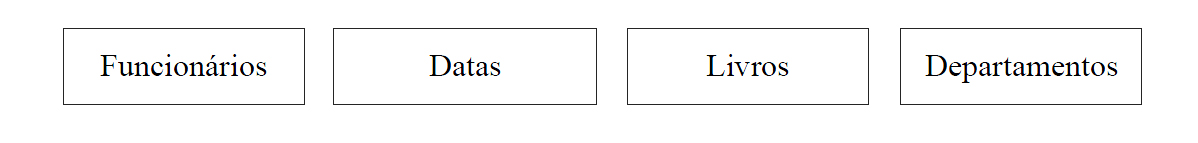
\includegraphics[width=11cm]{images/entidades.jpg}
        \end{center}
    \end{figure}
\end{frame}


\begin{frame}
    \frametitle{Entidades e conjuntos de entidades}
    \begin{block}{Caracteriza��o}
        \begin{itemize}
            \item Entidade: objeto que existe e que � distingu�vel de outros objetos $\Rightarrow$ Pode ser concreta ou
            abstrata.
            \item Conjunto de entidades: Conjunto de todas as entidades de um mesmo tipo.
        \end{itemize}
    \end{block}
    \begin{figure}[htb]
        \begin{center}
            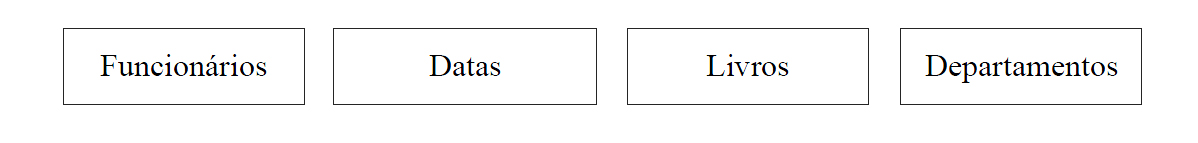
\includegraphics[width=11cm]{images/entidades.jpg}
        \end{center}
    \end{figure}
\end{frame}

\subsection{Atributos}

\begin{frame}
    \frametitle{Atributos}
    \begin{block}{Caracteriza��o}
        Permitem a associa��o de informa��es pertinentes aos "objetos"{} do
        mundo real.
    \end{block}
    \begin{figure}[htb]
        \begin{center}
            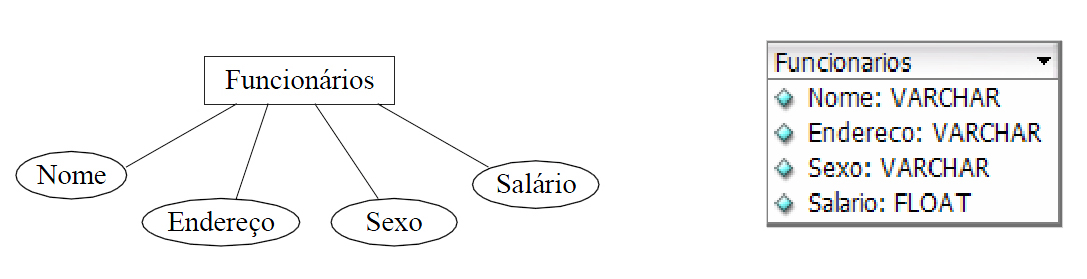
\includegraphics[width=10cm]{images/atributos.jpg}
        \end{center}
    \end{figure}
\end{frame}

\subsubsection{Atributos Compostos e Multivalorados}

\begin{frame}
    \frametitle{Atributos Compostos e Multivalorados}
    Atributos compostos:
    \begin{figure}[htb]
        \begin{center}
            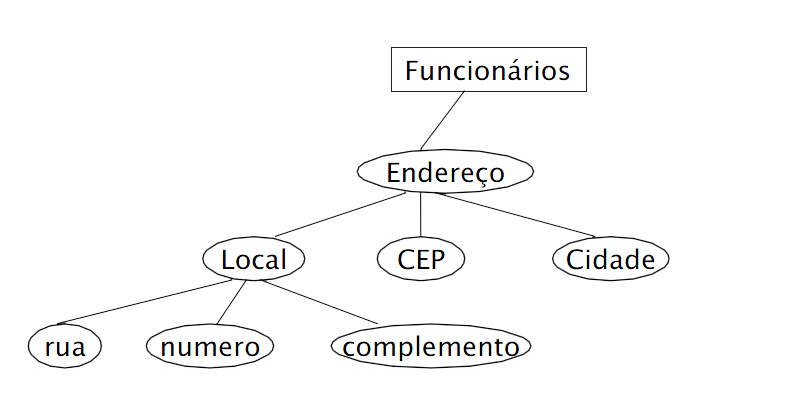
\includegraphics[width=6cm]{images/atributocomposto.jpg}
        \end{center}
    \end{figure}
    Atributos multivalorados:
    \begin{figure}[htb]
        \begin{center}
            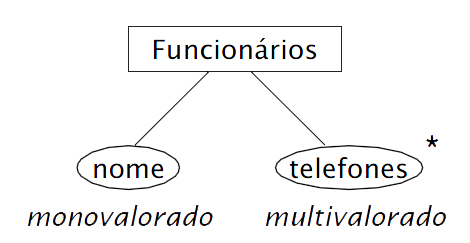
\includegraphics[width=4cm]{images/atributomultivalorado.jpg}
        \end{center}
    \end{figure}
\end{frame}

\subsection{Identificadores}

\begin{frame}
    \frametitle{Identificadores}
    \begin{block}{Caracteriza��o}
        Atributos que fornecem um nome ou identificam as inst�ncias da
        entidade.
    \end{block}
    \begin{itemize}
        \item �nico. Ex: num\_matr�cula\_funcionario;
        \item N�o �nico. Ex: nome\_funcionario;
        \item Composto. Ex: nome, num\_matricula;
    \end{itemize}
\end{frame}


\subsubsection{Super Chave}

\begin{frame}
    \frametitle{Superchave}
    \begin{block}{Caracteriza��o}
        Uma superchave � um conjunto de um ou mais atributos que identifica
        unicamente uma entidade.
    \end{block}
    \begin{figure}[htb]
        \begin{center}
            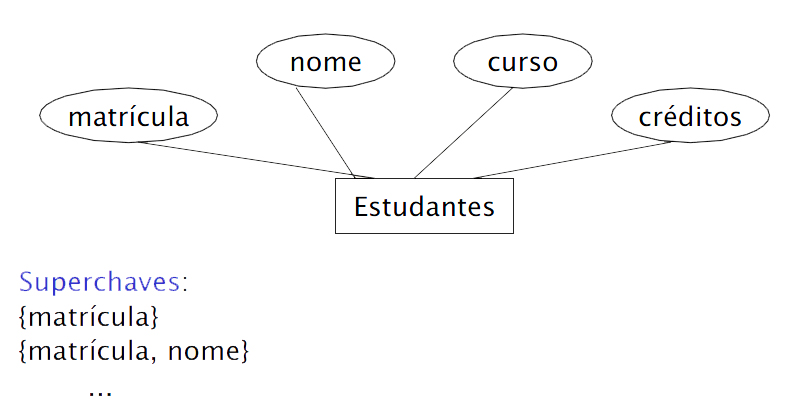
\includegraphics[width=8cm]{images/superchave.jpg}
        \end{center}
    \end{figure}
\end{frame}

\subsubsection{Chave Candidata}

\begin{frame}
    \frametitle{Chave Candidata}
    \begin{block}{Caracteriza��o}
        Uma chave candidata � uma superchave que n�o contem nenhum
        subconjunto pr�prio que seja por si s� uma superchave.
    \end{block}
    \begin{figure}[htb]
        \begin{center}
            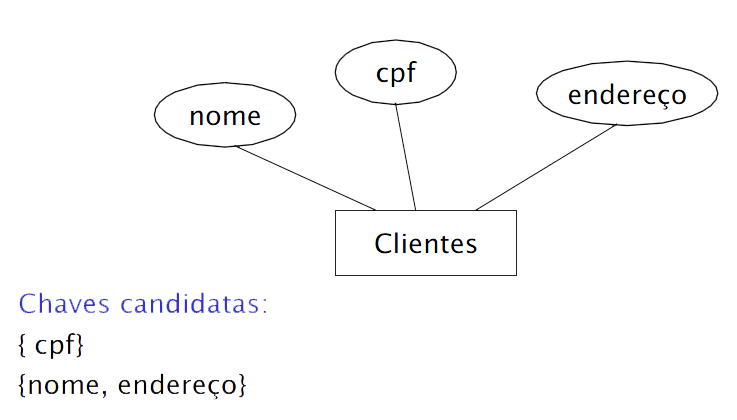
\includegraphics[width=8cm]{images/chavecandidata.jpg}
        \end{center}
    \end{figure}
\end{frame}

\subsubsection{Chave Prim�ria}

\begin{frame}
    \frametitle{Chave Prim�ria}
    \begin{block}{Caracteriza��o}
        Chave candidata escolhida pelo projetista do BD como principal meio
        de identifica��o de cada uma das entidades de um conjunto de
        entidades.
    \end{block}
    \begin{figure}[htb]
        \begin{center}
            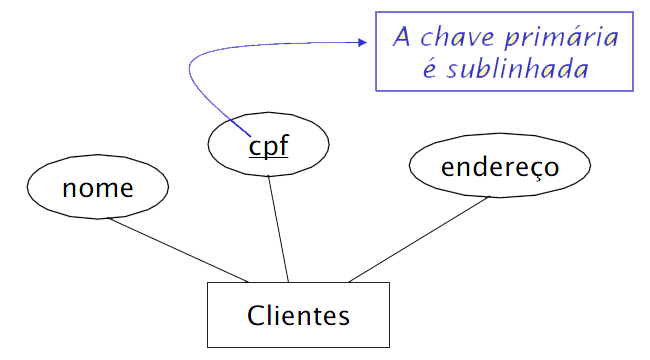
\includegraphics[width=6cm]{images/chaveprimaria.jpg}
        \end{center}
    \end{figure}
\end{frame}

\subsection{Relacionamentos}

\begin{frame}
    \frametitle{Relacionamentos}
    \begin{block}{Caracteriza��o}
        Associa��o entre v�rias entidades.
    \end{block}
    \begin{figure}[htb]
        \begin{center}
            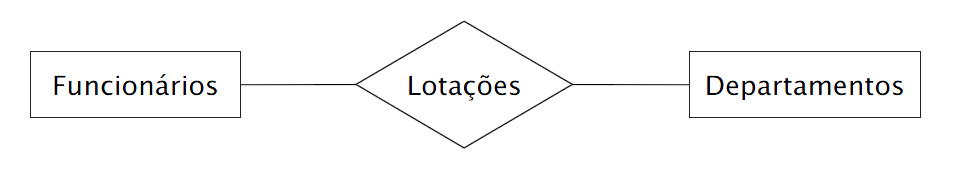
\includegraphics[width=10cm]{images/relacionamentos.jpg}
        \end{center}
    \end{figure}
\end{frame}

\subsection{Grau de Relacionamento}

\begin{frame}
    \frametitle{Cardinalidade do Mapeamento}
    \begin{itemize}
        \item Um-para-um (1:1);
        \item Um-para-muitos (1:n);
        \item Muitos-para-muitos (n:n);
    \end{itemize}
\end{frame}

\subsubsection{Cardinalidade do Mapeamento: 1:1}
\begin{frame}
    \frametitle{Cardinalidade do Mapeamento: 1:1}
    \begin{block}{Caracteriza��o}
        Uma entidade em A � associada com no m�ximo uma entidade em B e vice-versa.
    \end{block}
    \begin{figure}[htb]
        \begin{center}
            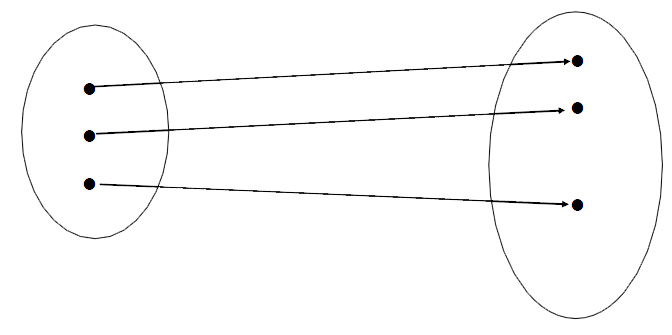
\includegraphics[width=6cm]{images/1p1.jpg}
        \end{center}
    \end{figure}
\end{frame}

\begin{frame}
    \frametitle{Diagramas de Exemplo}
    \begin{figure}[htb]
        \begin{center}
            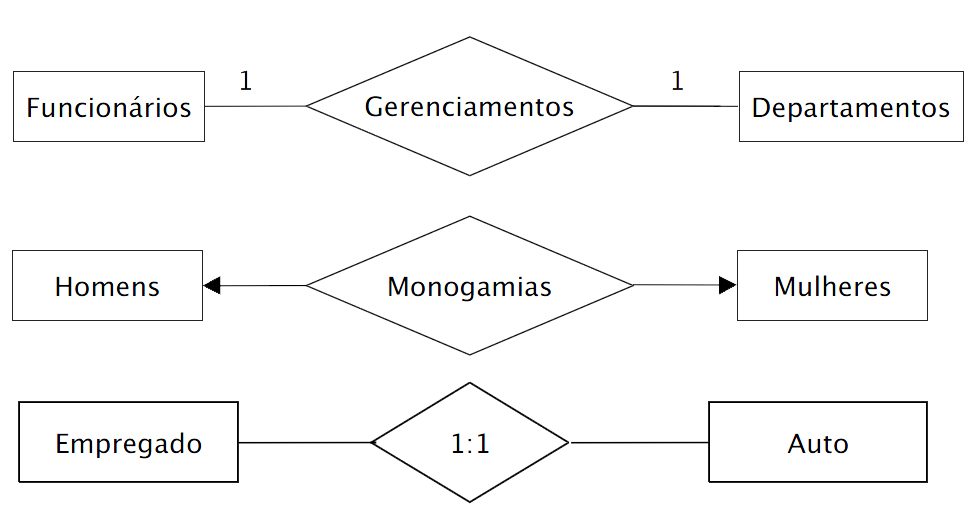
\includegraphics[width=10cm]{images/1p1e.jpg}
        \end{center}
    \end{figure}
\end{frame}

\subsubsection{Cardinalidade do Mapeamento: 1:N}
\begin{frame}
    \frametitle{Cardinalidade do Mapeamento: 1:N}
    \begin{block}{Caracteriza��o}
    Uma entidade de A � associada a qualquer n�mero de entidades de B, uma entidade de B, por outro lado, pode estar associada somente a uma entidade de
    A.
    \end{block}
    \begin{figure}[htb]
        \begin{center}
            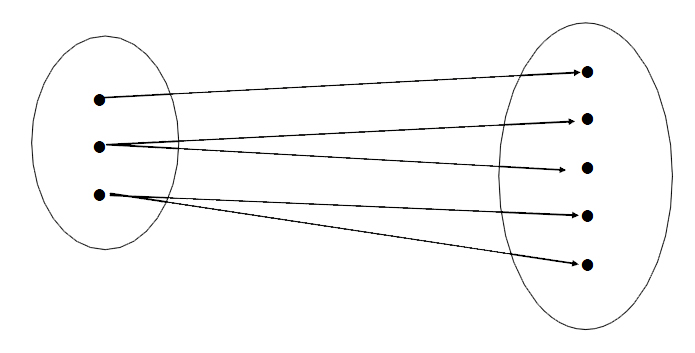
\includegraphics[width=6cm]{images/1pn.jpg}
        \end{center}
    \end{figure}
\end{frame}

\begin{frame}
    \frametitle{Diagramas de Exemplo}
    \begin{figure}[htb]
        \begin{center}
            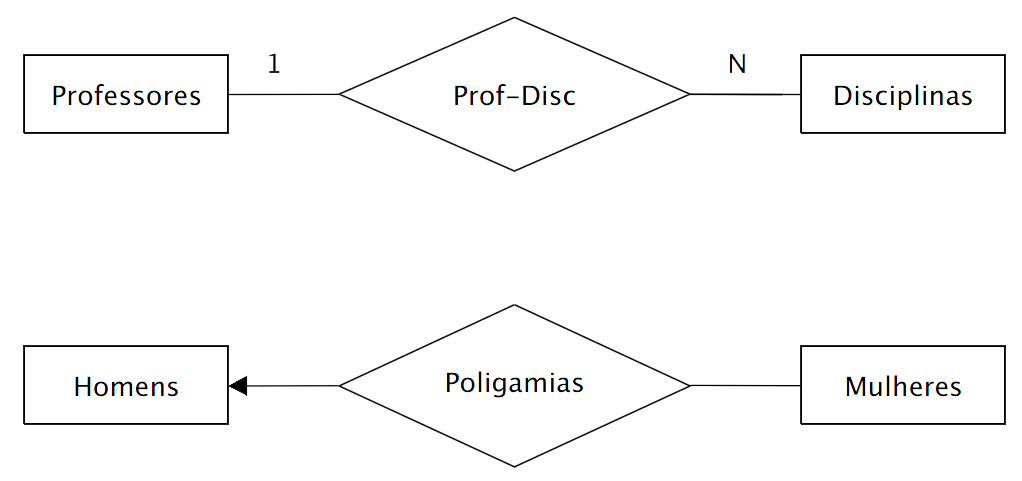
\includegraphics[width=10cm]{images/1pne.jpg}
        \end{center}
    \end{figure}
\end{frame}

\subsubsection{Cardinalidade do Mapeamento: N:N}
\begin{frame}
    \frametitle{Cardinalidade do Mapeamento: N:N}
    \begin{block}{Caracteriza��o}
        Uma entidade de A pode estar associada a qualquer n�mero de
        entidades de B e vice-versa.
    \end{block}
    \begin{figure}[htb]
        \begin{center}
            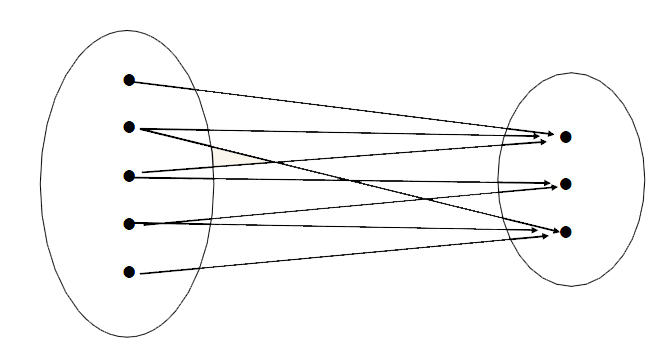
\includegraphics[width=6cm]{images/npn.jpg}
        \end{center}
    \end{figure}
\end{frame}

\begin{frame}
    \frametitle{Diagramas de Exemplo}
    \begin{figure}[htb]
        \begin{center}
            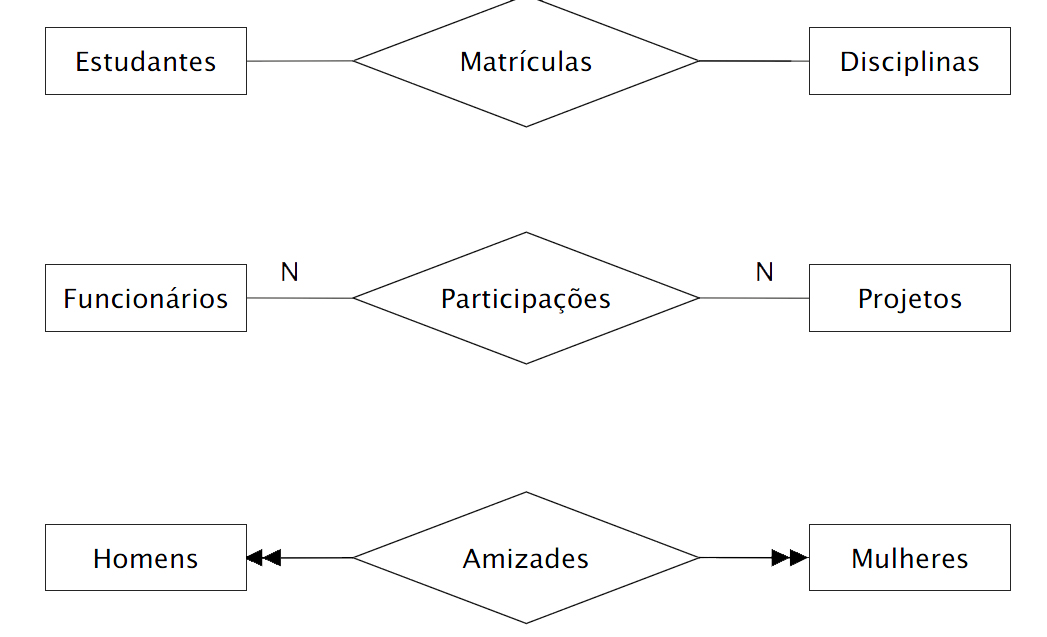
\includegraphics[width=10cm]{images/npne.jpg}
        \end{center}
    \end{figure}
\end{frame}

\section[Postgres]{Postgres}
\begin{frame}
    \frametitle{Uma breve hist�ria do PostGreSQL}
    \begin{itemize}
        \item Banco de dados objeto-relacional;
        \item Derivado do pacote POSTGRES (Universidade da Calif�rnia em
        Berkeley);
        \begin{itemize}
            \item 1986 in�cio do projeto;
            \item 1987 primeira vers�o do Postgres;
            \item 1989 libera��o para usu�rios restritos da vers�o 1;
            \item 1991 vers�o 3 com as principais funcionalidades atuais;
            \item 1993 vers�o 4.2, �ltima lan�ada pela Berkeley;
            \item 1994 Andrew Yu e Jolly Chen criaram a vers�o conhecida como Postgre95 com interpretador para a linguagem SQL;
            \item 1997 Nome do projeto muda para PostgreSQL, a vers�o 6 � lan�ada;
            \item 2000 vers�o 7 lan�ada com suporte a Foreign Key;
            \item 2005 vers�o 8 lan�ada com vers�o nativa (sem uso do CYGWIN) para Windows, TABLESPACES, SAVEPOINTS, POINTINTIMERECOVERY. etc.
        \end{itemize}
    \end{itemize}
\end{frame}

\subsection{ACID}
\begin{frame}
    \frametitle{ACID}
    \begin{itemize}
        \item \emph{Atomicidade}: transa��es n�o podem ficar pela metade (tudo ou nada);
        \item \emph{Consist�ncia}: transa��es devem transformar um estado consistente do banco em outro estado consistente;
        \item \emph{Isolamento}: transa��es s�o isoladas umas das outras, elas n�o "enxergam"{} dados gravados por transa��es concorrentes;
        \item \emph{Durabilidade}: uma vez efetuada a transa��o os dados devem permanecer no banco.
    \end{itemize}
\end{frame}

\subsection{Alguns tipos de dados}
\begin{frame}
    \frametitle{Alguns tipos de dados}
    \begin{figure}[htb]
        \begin{center}
            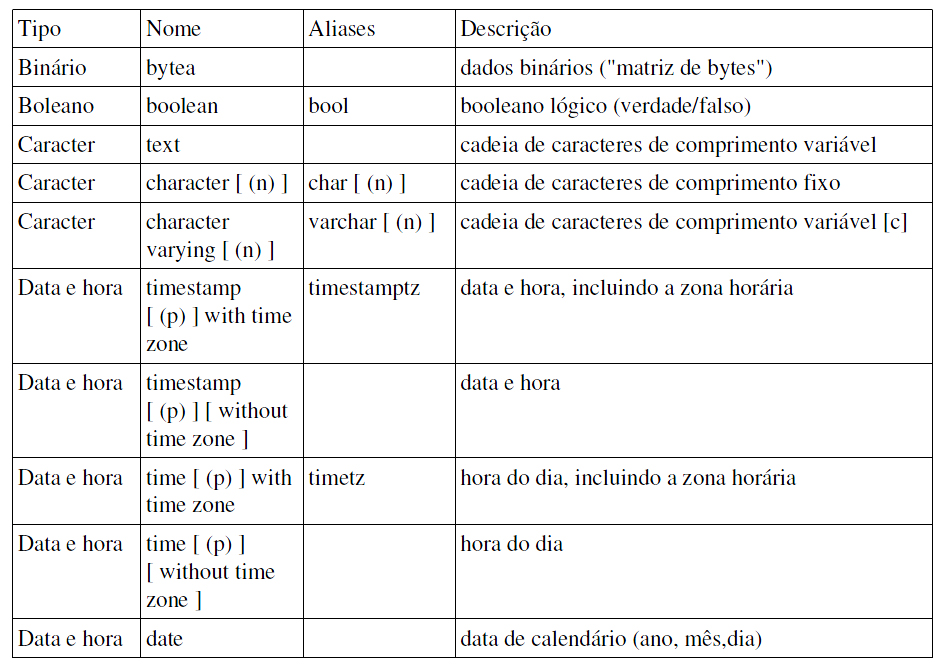
\includegraphics[width=9cm]{images/td1.jpg}
            \caption{Alguns tipos de dados}
        \end{center}
    \end{figure}
\end{frame}

\begin{frame}
    \frametitle{Alguns tipos de dados II}
    \begin{figure}[htb]
        \begin{center}
            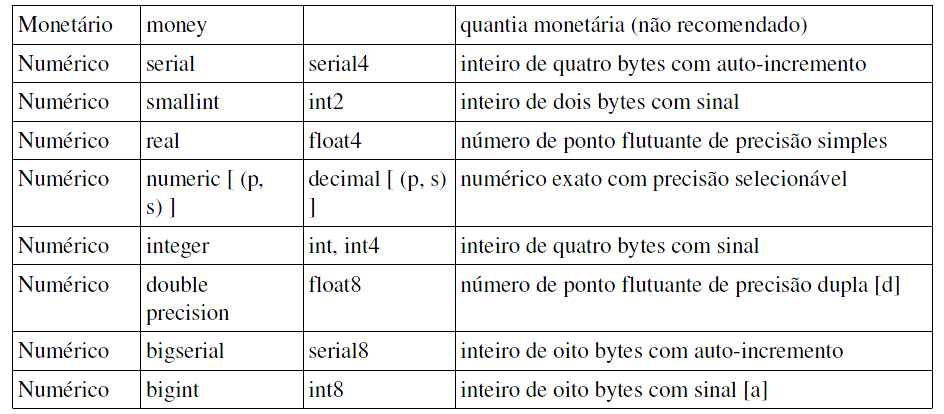
\includegraphics[width=9cm]{images/td2.jpg}
            \caption{Alguns tipos de dados}
        \end{center}
    \end{figure}
\end{frame}

\subsection{Funcionalidades Avan�adas}
\begin{frame}
    \frametitle{No PostgreSQL voc� pode:}
    \begin{itemize}
        \item Criar valida��es de dados;
        \item Criar tipos de dados personalizados;
        \item Disparar \emph{stored procedures} a partir de eventos das tabelas;
        \item Dividir o banco de dados em esquemas;
        \item Alocar bases inteiras, esquemas ou tabelas em locais diferentes (disco ou
        rede);
    \end{itemize}
\end{frame}

\begin{frame}
    \frametitle{Componentes do PostgreSQL:}
    \begin{itemize}
        \item Esquemas;
        \item Heran�a;
        \item Views;
        \item Fun��es;
        \item Restri��es;
        \item Gatilhos;
    \end{itemize}
\end{frame}

\subsection{Linguagem de Defini��o de Dados(DDL)}

\subsubsection{Create Table}
\begin{frame}[t,allowframebreaks]
    \frametitle{Create Table}
    Utilizado para criar tabelas.
    \texttt{\lstinputlisting[language=C, label=createtable,
    caption={Sintaxe da linguagem DDL para cria��o de tabelas}]{cods/createtable.txt}}
\end{frame}

\begin{frame}
    \frametitle{Usando corretamente o Create Table}
    \texttt{\lstinputlisting[language=C, label=createtable1,
    caption={Boa pr�tica usando Create Table}]{cods/createtable1.txt}}
\end{frame}

\begin{frame}
    \frametitle{Usando o Create Table sem conven��o}
    \texttt{\lstinputlisting[language=C, label=createtable2,
    caption={M� pr�tica usando Create Table}]{cods/createtable2.txt}}
\end{frame}

\subsubsection{Alter Table}
\begin{frame}[t,allowframebreaks]
    \frametitle{Alter Table}
    Utilizado para alterar tabelas.
    \texttt{\lstinputlisting[language=C, label=altertable,
    caption={Sintaxe da linguagem DDL para altera��o de tabelas}]{cods/altertable.txt}}
\end{frame}

\subsubsection{Drop Table}
\begin{frame}
    \frametitle{Drop Table}
    Remove uma ou mais tabelas.
    \texttt{\lstinputlisting[language=C, label=droptable,
    caption={Sintaxe da linguagem DDL para remover tabelas}]{cods/droptable.txt}}
\end{frame}

\subsubsection{Comment}
\begin{frame}
    \frametitle{Comment}
    Adiciona coment�rios em uma tabela, coluna, indice, restri��o, fun��o, indice, etc.
    \texttt{\lstinputlisting[language=C, label=comment,
    caption={Sintaxe da linguagem DDL para fazer coment�rios}]{cods/comment.txt}}
\end{frame}

\subsubsection{Create Index}
\begin{frame}
    \frametitle{Create Index}
    Cria um �ndice numa tabela.
    \texttt{\lstinputlisting[language=C, label=comment,
    caption={Sintaxe da linguagem DDL para criar �ndices}]{cods/index.txt}}
\end{frame}

\subsection{Linguagem de Modifica��o de Dados (DML)}

\subsubsection{Insert}
\begin{frame}
    \frametitle{Insert}
    Insere um registro em uma tabela.
    \texttt{\lstinputlisting[language=C, label=insert,
    caption={Sintaxe da linguagem DML para inserir registro}]{cods/insert.txt}}
\end{frame}

\subsubsection{Update}
\begin{frame}
    \frametitle{Update}
    Atualiza um registro em uma tabela.
    \texttt{\lstinputlisting[language=C, label=update,
    caption={Sintaxe da linguagem DML para atualizar registro}]{cods/update.txt}}
\end{frame}

\subsubsection{Delete}
\begin{frame}
    \frametitle{Delete}
    Remove um registro em uma tabela.
    \texttt{\lstinputlisting[language=C, label=delete,
    caption={Sintaxe da linguagem DML para remover registro}]{cods/delete.txt}}
\end{frame}

\subsubsection{Truncate}
\begin{frame}
    \frametitle{Truncate}
    Zera os registros de uma tabela.
    \texttt{\lstinputlisting[language=C, label=truncate,
    caption={Sintaxe da linguagem DML para zerar os registros de uma tabela}]{cods/truncate.txt}}
\end{frame}

\section[Subconsultas e Jun��es]{Subconsultas e Jun��es}

\subsection{Exists}
\begin{frame}
    \frametitle{Exists}
    \begin{block}{Caracteriza��o}
        Verifica se um valor existe no \emph{resultset} retornado por um
        \emph{select}.
    \end{block}
    \begin{itemize}
        \item Se a subconsulta retornar pelo menos uma linha, o resultado dela � TRUE, caso contr�rio ser�
        FALSE;
        \item Observe a liga��o entre a consulta externa e a
        interna.
    \end{itemize}
    \texttt{\lstinputlisting[language=C, label=exists,
    caption={Exemplo de utiliza��o do Exists}]{cods/exists.txt}}
\end{frame}

\subsection{In e Not In}
\begin{frame}
    \frametitle{In e Not In}
    \begin{block}{Caracteriza��o}
        Verifica  se um valor est� contido em um grupo de valores.
    \end{block}
    \texttt{\lstinputlisting[language=C, label=innotin,
    caption={Exemplo de utiliza��o do in e not in}]{cods/innotin.txt}}
\end{frame}

\begin{frame}
    \frametitle{Formas Alternativas para In e Not In}
    \texttt{\lstinputlisting[language=C, label=innotinalt,
    caption={Exemplo de utiliza��o do in e not in de formas alternativas}]{cods/innotinalt.txt}}
\end{frame}

\subsection{Jun��es}
\subsubsection{Inner Join}
\begin{frame}
    \frametitle{Inner Join}
    \begin{block}{Caracteriza��o}
        Somente as linhas/registros que satisfa�am a liga��o determinada
        pelo \emph{JOIN} ser�o recuperados pelo \emph{SELECT}, sendo assim, os registros
        que n�o se enquadram no relacionamento definido pelo \emph{JOIN} n�o ser�o
        recuperados.
    \end{block}
\end{frame}

\begin{frame}
    \frametitle{Exemplo}
    \texttt{\lstinputlisting[language=C, label=innerjoin,
    caption={Exemplo de utiliza��o do Inner Join}]{cods/innerjoin.txt}}
\end{frame}

\subsubsection{Left Join}
\begin{frame}
    \frametitle{Left Join}
    \begin{block}{Caracteriza��o}
        Atrav�s do uso do \emph{LEFT}, todos os registros na tabela � esquerda da
        \emph{query} ser�o listados, independente de terem ou n�o registros
        relacionados na tabela � direita. Nesse caso, as colunas
        relacionadas com a tabela da direita voltam nulos (\emph{NULL}).
    \end{block}
\end{frame}

\begin{frame}
    \frametitle{Exemplo}
    \texttt{\lstinputlisting[language=C, label=leftjoin,
    caption={Exemplo de utiliza��o do Left Join}]{cods/leftjoin.txt}}
\end{frame}

\subsubsection{Right Join}
\begin{frame}
    \frametitle{Left Join}
    \begin{block}{Caracteriza��o}
        � o inverso do \emph{Left Join}, ou seja, todos os registros da tabela �
        direita ser�o listados, independente de terem ou n�o registros relacionados na tabela � esquerda.
    \end{block}

\end{frame}

\begin{frame}
    \frametitle{Exemplo}
    \texttt{\lstinputlisting[language=C, label=rightjoin,
    caption={Exemplo de utiliza��o do Right Join}]{cods/rightjoin.txt}}
\end{frame}


\end{document}
